%%%%%%%%%%%%%%%%%%%%%%%%%%%%%%%%%%%%%%%%%%%%%%%%%%%%%%%%%%%%%%%%%%%%%
% LaTeX Template: Project Titlepage Modified (v 0.1) by rcx
%
% Original Source: http://www.howtotex.com
% Date: February 2014
% 
% This is a title page template which be used for articles & reports.
% 
% This is the modified version of the original Latex template from
% aforementioned website.
% 
%%%%%%%%%%%%%%%%%%%%%%%%%%%%%%%%%%%%%%%%%%%%%%%%%%%%%%%%%%%%%%%%%%%%%%

\documentclass[12pt]{article}
\usepackage[a4paper]{geometry}
\usepackage[myheadings]{fullpage}
\usepackage{fancyhdr}
\usepackage{lastpage}
\usepackage{graphicx, wrapfig, subcaption, setspace, booktabs}
\usepackage[T1]{fontenc}
\usepackage[font=small, labelfont=bf]{caption}
\usepackage{fourier}
\usepackage[protrusion=true, expansion=true]{microtype}
\usepackage[english]{babel}
\usepackage{sectsty}
\usepackage{url, lipsum}
\usepackage{tabularx}
\usepackage{textcomp}
\usepackage{amsmath}
\usepackage{float}

\newcommand\boldblue[1]{\textcolor{blue}{\textbf{#1}}}
\newcommand{\HRule}[1]{\rule{\linewidth}{#1}}
\onehalfspacing
\setcounter{tocdepth}{5}
\setcounter{secnumdepth}{5}

%-------------------------------------------------------------------------------
% HEADER & FOOTER
%-------------------------------------------------------------------------------
\pagestyle{fancy}
\fancyhf{}
\setlength\headheight{15pt}
\fancyhead[L]{CHARM}
\fancyhead[R]{Carleton University}
\fancyfoot[R]{Page \thepage\ of \pageref{LastPage}}
%-------------------------------------------------------------------------------
% TITLE PAGE
%-------------------------------------------------------------------------------

\begin{document}
\bibliographystyle{ieeetr}

\title{ \normalsize \textsc{}
		\\ [2.0cm]
		\HRule{0.5pt} \\
		\LARGE \textbf{{Carleton High Altitude Radiometer}}\\
		\large \textbf{{Project Proposal}}\\
		\large \textbf{{Canadian Stratospheric Balloon Experiment Design Challenge}}
		\HRule{2pt} \\ [0.5cm]
		\normalsize \today \vspace*{2\baselineskip}\\
		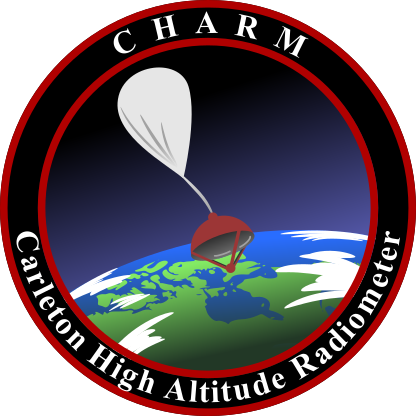
\includegraphics[scale=0.6]{Figures/CHARM.png}	\vspace*{2\baselineskip} \\
		\textsc{
		Jacob Booth \\
		David Bascelli \\
		}}
		
\date{}
	
\author{
		Carleton University \\
		}
	


\maketitle

\newpage

\tableofcontents
\newpage

\listoffigures
\newpage

\listoftables
\newpage

%-------------------------------------------------------------------------------
% Section title formatting
\sectionfont{\scshape}
%-------------------------------------------------------------------------------

%-------------------------------------------------------------------------------
% BODY
%-------------------------------------------------------------------------------

\section{Executive Summary}
Microwave remote sensors have been a common payload on earth observation satellites since the early days of space-flight. In as early as 1962, a passive radiometer on-board the Mariner 2 mission measured the surface temperature of Venus. 1968 Saw the first space-born earth observation radiometer on-board the Cosmos 243 satellite, which measured atmospheric water vapour and global ice cover. Many different radiometer configurations can make a wide array of different geological, biological, and climate measurements. The Carleton High Altitude RaidioMeter project (CHARM) will design and manufacture a balloon mounted microwave radiometer for the purpose of measuring soil moisture content over a large area. Soil moisture measurements are crucial in predicting local weather conditions and monitoring climate change. Incorporating soil moisture measurements into weather and climate models allows for more accurate medium term weather forecasts and can also give clues about future droughts, crop yields, and water resource management. Soil moisture measurements have also been used to predict wildfire risk. Currently, most radiometric data comes from space-born radiometers, such as those on the SMAP or SMOS satellites. To achieve high resolution and accuracy, these space-born radiometers utilize cryogenic components, complex phased array or synthetic aperture technologies, and require large and very directional antennas. Our belief is that measurements of similar similar quality could be performed from a high altitude balloon at significantly reduced cost. 

\newpage

\section{Proposal}
\subsection{Scientific Objective}

Our scientific objective is to make low cost measurements of soil moisture content using a balloon born passive microwave radiometer. The payload will take wide-band measurements of the microwave noise emitted by the ground and determine soil moisture content through a modification of the zeroth order radiative transfer model (ZRT Model). A basic dielectric model will be used to solve for volumetric moisture content. \cite{ulaby_fung_moore_1986} A NADIR pointing antenna will extend from the pelican case to take measurements of the background microwave emissions coming from the ground. The radiometer will be of the hybrid type, which directly digitizes antenna readings for digital processing. A 9-axis inertial measurement unit (IMU) will measure linear acceleration, angular rates, and magnetic field strength to determine the attitude of the payload. GPS data will be saved to track the location of the payload as it passes over the earth. With the attitude and GPS data, a map of soil moisture content under the payloads flight path will be able to be made. 

A Balloon born microwave radiometer to measure soil moisture was selected for several reasons. First, soil moisture content was chosen to be measured because of its importance to weather and climate monitoring.\cite{Pan2001} Climate models, weather predictions, crop yield estimation and water resource management systems all benefit from accurate and up to date measurements of ground moisture content. Soil moisture measurements have also proved useful in predicting wildfires.\cite{chaparro_piles_vall-llossera_2016,krueger_ochsner_quiring_engle_carlson_twidwell_fuhlendorf_2017} Second, measuring soil moisture content from radiometers is reasonably common, and as such a significant amount of literature exists on the topic. Most literature either concerns satellite born radiometers, aircraft born radiometers, or static ground based radiometers. \cite{Hanington,Kerr2001,ulaby_fung_moore_1986,Friesen2008,Schmugge1994} By exploring the possibility of balloon based radiometers and by attempting more advanced soil moisture estimation techniques, we can achieve a degree of novelty while still having a wealth of proven literature and designs to aid us. Third, balloon mounted radiometers have several advantages to static, aircraft mounted, and satellite radiometers. Due to the balloon's proximity to the ground compared to low earth orbit, balloon born radiometers can achieve greater resolution with smaller and less directional antennas. Balloon radiometers can achieve much greater loiter times than aircraft mounted radiometers, although balloons are uncontrolled. Balloon born radiometers also have the advantage of being significantly cheaper to operate than aircraft or satellite mounted radiometers. A trade study was performed in table \ref{tab:vehicle_trade}, and it can be seen that balloon born radiometers offer a unique performance compromise at very low cost when compared to aircraft mounted or satellite based radiometers.

\begin{table}[!h]
	\centering
	\vspace{0.5cm}
	\renewcommand{\arraystretch}{1.3}
	\caption{Radiometer Vehicle Trade Study. }
	\label{tab:vehicle_trade}
	\begin{tabularx}{\textwidth}{llll}
		\toprule
						& Satellite & Aircraft & Balloon \\		
		\midrule
		Cost					&Very High&Moderate&Low \\ 
		Antenna Size 			&Large&Small&Small/Medium \\
		Resolution 				&Low Resolution&High Resolution&Medium Resolution \\ 
		Atmospheric Effects		&High&Low&Moderate \\ 
		Loiter Time				&N/A&Up to 6 hours&6 - 48 Hours \\ 
		Controllability			&Uncontrolled but predictable&Controlled&Uncontrolled 
	\end{tabularx}
\end{table}

Lastly, soil moisture retrieval from radiometric data is one of the more simple radiometer configurations to design and operate, allowing our team to gain experience with radiometer principals before attempting more advanced designs. Thus, a microwave radiometer was chosen as our balloon payload because of its many geoscientific applications, the wealth of literature and design aids, their suitability to the high altitude balloon environment, and because it allows us to gain experience with a relatively simple radiometer configuration.
 
\subsection{Experiment Design}

Passive microwave radiometers work by measuring the natural electromagnetic radiation emissions from the earth's surface in the microwave band. Liquid water content and water vapour is translucent to microwave frequencies, so an estimation of soil water content can be made by measuring the power of the emitted noise. By utilizing modern digital signal processing techniques, a wide-band power spectral density of the noise will be calculated. Using a radiative transfer model and by utilizing tertiary data-sets, the power spectral density of the microwave noise will be able to give a measurement of soil moisture content.

\subsubsection{Radiometer Block Diagram}

There are many different kinds of radiometer systems, but for this experiment we choose to implement a hybrid radiometer \cite{skou1989microwave}. A hybrid design was chosen because it requires the simplest analog front end, at the expense of greater complexity in the digital signal processing. This is a relatively new design made possible by monolithic integrated circuits that allow small and high speed analog to digital converters (ADC) and powerful digital signal processors. A hybrid radiometer essentially consists of a microwave amplifier and a superheterodyne receiver. The downsampled signals are then sampled by an ADC. This is far less complicated then the more traditional Dicke radiometer, which contains analog detector and integrator stages before the ADC. 

A high level diagram of our system is shown in figure \ref{fig:system_diagram}. It contains an antenna as described in section \ref{sec:antenna}, an analog front end, and a digital signal processor. The digital signal processor will be implemented on an field programmable gate array (FPGA) attached to our motherboard.

A overview of the analog front end is given in figure \ref{fig:analog_diagram}, this will be implemented an a PCB that is made with a special RF grade low loss dielectric. It will be built as a daughter card that attaches to the same motherboard as the FPGA.

The analog system contains a switch at the front which rapidly switches between the antenna and a known noise reference. This allows the system to get a differential measurement and thus eliminates variable gain in the amplifier as a source of error. The analog system also contains amplifiers and filters to avoid aliasing and other effects.

\begin{figure}
	\centering
	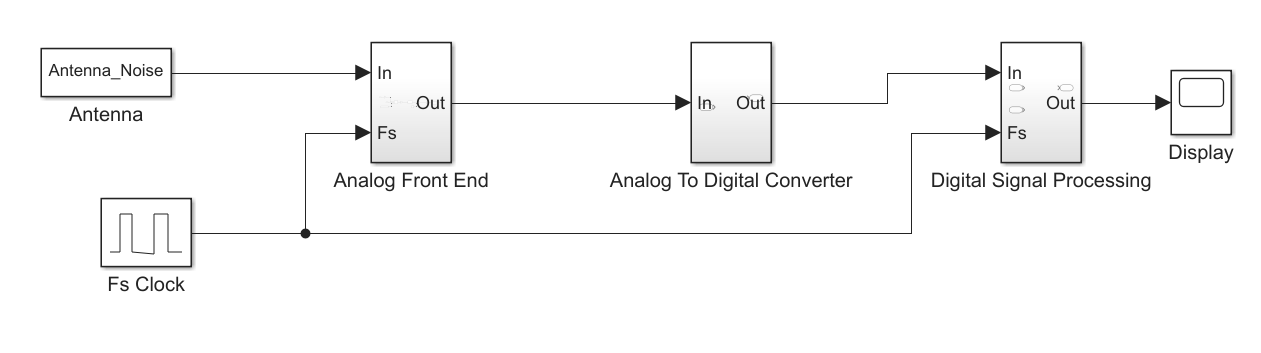
\includegraphics[width=\linewidth]{Figures/radiometer_system.png}
	\caption{Block diagram of radiometer system design}
	\label{fig:system_diagram}
\end{figure}

\begin{figure}
	\centering
	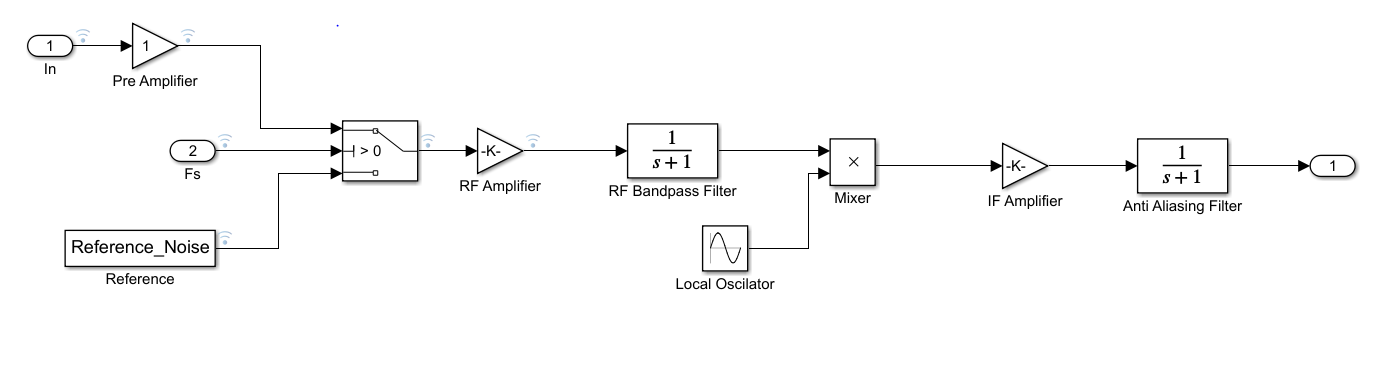
\includegraphics[width=\linewidth]{Figures/analog_front_end.png}
	\caption{Block diagram of analog front end}
	\label{fig:analog_diagram}
\end{figure}



\subsubsection{Antenna Selection and Fabrication} \label{sec:antenna}

The design and construction of the antenna system presents many challenges. It is desired that the antenna be highly directional, which typically requires them to be quite large and heavy. A highly directional antenna allows a greater ground resolution and thus a detailed soil moisture map can be extracted. It should also be noted that lower frequencies require larger antennas. Therefore, antenna sizing is the defining constraint on this system. There are two solutions under consideration for the design of the antenna. A single large antenna, or an antenna array. Using an array of radiometers, we can create a synthetic aperture radiometer (SAR). With this solution we would likely measure at 1.4 GHz, reducing hardware expense and complexity. This would involve precisely placing four to eight antennas around the base of the gondola. The individual antennas would only be 10 cm long, and weigh very little. Coax cable would then need to be routed back to the experiment case. The use of SAR is common in space based installations, as it is far lighter then having a single large dish \cite{skou1989microwave}. However, the placement of many antennas, and the routing of many cables through the gonadal would be problematic. In addition the signal processing required to get meaningful data from a SAR is incredibly complex and difficult, making this solution undesirable. It is mentioned here in the event that the second solution does not work. 

The second solution is to use a single large horn antenna which protrudes from the side of the gonadal as shown in figure \ref{fig:antenna}. While this has the advantage of being easier to implement and build, it is heavier and less directional. The exact sizing of the antenna would have to be carefully chosen to be as large as allowable to provide the best possible ground resolution. The horn antenna will contain two outputs to allow the measurement of the polarization of the incident radiation\cite{constantine2005antenna}. Being able to take these simultaneous measurements can eliminate one of the variables required to extract soil moisture data.

\begin{figure}
	\centering
	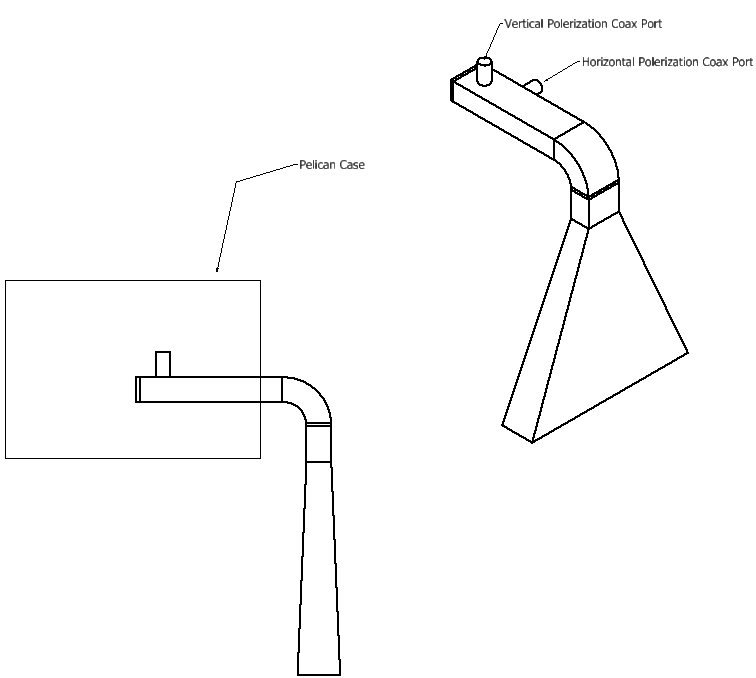
\includegraphics[width=0.5\linewidth]{Figures/rough_antenna.png}
	\caption{Horn antenna}
	\label{fig:antenna}
\end{figure}

The graph shown in figure \ref{fig:antenna_direction} shows the directivity of the antenna shown in figure \ref{fig:antenna}.

\begin{figure}
	\centering
	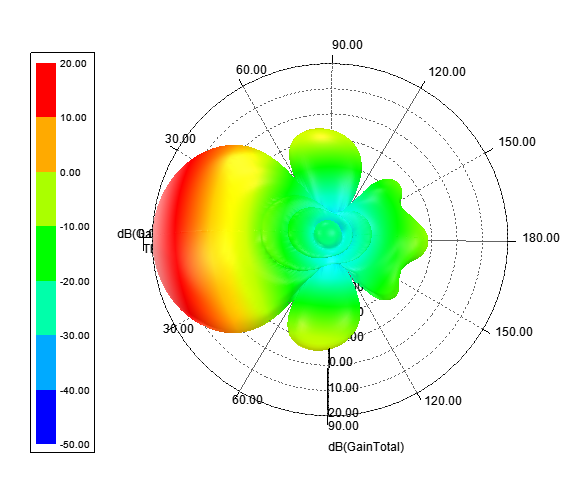
\includegraphics[width=0.5\linewidth]{Figures/antenna_gain.png}
	\caption{Horn antenna directivity}
	\label{fig:antenna_direction}
\end{figure}

One way of constructing the antenna is to have large copper sheets cut into shape then soldered together. While this is fairly easy, it is imprecise and the resulting antenna may have poor performance. Another solution being investigated is 3D printing the antenna and then electroplating it in copper. This will allow us to create more complicated geometry and be much lighter then something made of solid copper. In house electroplating is being investigated for  reduced cost, but the process in difficult and requires the development of procedures and techniques \cite{bryancera2014}. Alternatively, a third party can be hired to electroplate our 3D print.

\subsubsection{Microwave Band Selection}

Most soil moisture radiometers make use of L-band measurements (1-2 GHz), usually at or around 1.4 GHz. L-band measurements are ideal for soil moisture extraction for several reasons. First, the L-band is nearly transparent to vegetation, allowing for more accurate measurements. Second, the L-band penetrates up to a meter of soil, allowing deeper measurements. Deeper measurements may more accuratly represent true groundwater content. Third, there is a reserved band for radio-astronomy at 1.4 GHz, reducing potential sources of interference. Lastly, RF components in the L-band have become increasingly cheap due to commercial applications such as WiFi and cellular networks. Another advantage to choosing the L-band is that there is a significant amount of literature and proven L-Band radiometer designs and models. The L-band however requires large antennas or complex measurement techniques to achieve directional measurements and build a map of soil moisture content. For example the radiometer aboard the SMOS satellite uses aperture synthesis and three large antennas ~1 meter in length to achieve a ground resolution of 35-50 km from a 755km orbit. \cite{Wigneron2010}. The SMAP mission uses a 6 meter dish antenna to achieve 40 km ground resolution from a 685 km orbit. \cite{entekhabi_njoku_oneill_spencer_jackson_entin_im_kellogg_2008}  For our radiometer, even a 30 cm dish only achieves a beam-width of 45 degrees at 1.4 GHz. Due to the spacial requirements of the CAN-SBX competition, even a 30 cm antenna might be too large. Thus, currently radiometers in the C-band (4-8 GHz) are being explored. C-band radiometers share some of the benefits of L-band radiometers. Components are still quite cheap due to the prevalence of WiFi and Bluetooth technology, there are some reserved radio-astronomy bands within the C-band, and there is some recent literature concerning soil moisture estimation from C-band radiometers. \cite{Description2000,jackson_gasiewski_oldak_klein_njoku_yevgrafov_christiani_bindlish_2002} However, the C-band does not penetrate the ground as far and can only accurately measure soil moisture to around 10-20 cm depth. Atmospheric microwave emissions are slightly stronger at the C-band, making it more difficult to accurately determine soil moisture content. The C-band is more greatly effected by ground vegetation type, water content in the ground vegetation canopy, and surface roughness effects, making accurate measurements more difficult or impossible. \cite{ulaby_fung_moore_1986} However, C-band radiometers offer much smaller antennas and much higher directionality and ground resolution. The same 30 cm parabolic dish antenna would achieve a 10 degree beam-width, allowing a ground resolution of 5 km at an altitude of 30 km. Both L-band and C-band options are currently being considered for the radiometer. A trade study table can be seen in table \ref{tab:band_trade}.


\begin{table}[!h]
	\centering
	\vspace{0.5cm}
	\renewcommand{\arraystretch}{1.3}
	\caption{Radiometer Band Trade Study. }
	\label{tab:band_trade}
	\begin{tabularx}{\textwidth}{lXll}
		\toprule
									& & L-Band & C-Band \\		
		\midrule
		Frequency					& &1-2 GHz&4-8 GHz \\ 
		Component Cost				& &Low&Moderate	 \\
		Antenna Size 				& &Large&Small	 \\
		Resolution 					& &Low Resolution&High Resolution 	\\ 
		Atmospheric Emission		& &Low&Moderate 					\\ 
		Effect of Vegetation		& &Low&Moderate						\\
		Effect of Surface Roughness	& &Low&Moderate						\\
		Ground Penetration			& &Up to 1 meter&10-20 cm			\\
		Available Literature 		& &High&Moderate	
	\end{tabularx}
\end{table}

\subsubsection{Soil Moisture Transfer Model}

To extract soil moisture content from radiometric data, a model of the received noise power must be formed. There are several parameters other than the soil moisture content that contribute to the total noise power measured by a radiometer. Surface roughness, surface temperature, presence and type of vegetation, atmospheric conditions, and antenna incidence angle all greatly effect the measured noise power and must be isolated to return an accurate soil moisture measurement. Isolating the ground moisture content is usually performed either by knowing tertiary information about the observed surface, or by making multiple measurements at different incidence angles, polarities, or frequencies. Our radiometer will measure the power spectral density over a wide band, but essentially only a single measurement will be made to reduce cost and complexity. Our radiometer will therefore have to rely on tertiary information such as open on-line data-sets for earth ground cover, vegetation type, surface roughness, and surface temperature to eliminate several variables and obtain accurate measurements. Two methods are usually employed to solve for soil moisture content from the tertiary data and from the measured power spectral density.

\begin{enumerate}
\item Empirical models have been historically used to solve for soil moisture due to their computational simplicity. Several papers have performed experiments to determine models for various surface roughness's, vegetation types, and frequency ranges. These models can achieve accurate extraction of soil moisture content. Often though, these models are limited in scope due to the challenges in taking measurements over a a wide array of conditions. These models are also only suited for the specific instrument and measurements that the authors wish to make and are difficult to apply to a general case. Making our own empirical model is an option but would be time consuming and difficult.

\item Inverting a radiative transfer model allows the extraction of soil moisture content for any arbitrary radiometer, given that the parameters of the surface and atmosphere is well known at the desired frequency. This method is only as accurate as the ability to estimate the surface conditions and the applicability of the model to real world conditions. This method could introduce errors by ignoring some radiative effects or non-linearity's that an empirical model might be able to account for. Still, inverting a radiative transfer model allows for a more general solution that could by applied to any radiometric data. The zeroth order transfer function is the most basic function that has been used to extract soil moisture content and takes the form
\begin{align}
e_{veg}^p(\theta_i) = (1+\Gamma_{coh}^p(\theta_i)\Upsilon_{veg})(1-a)(1-\Upsilon_{veg})+\Upsilon_{veg}e_{soil}^p(\theta_i)
\end{align}
where
\begin{align}
e &= Emissivity\\
\theta_i &= Incidence Angle\\
p &= Antenna Polarization\\
\Upsilon &= Microwave Emission\\
\Gamma &= Microwave Reflection\\
a &= Vegitation Scattering Albedo
\end{align}

\begin{figure}[htbp!]
	\centering
	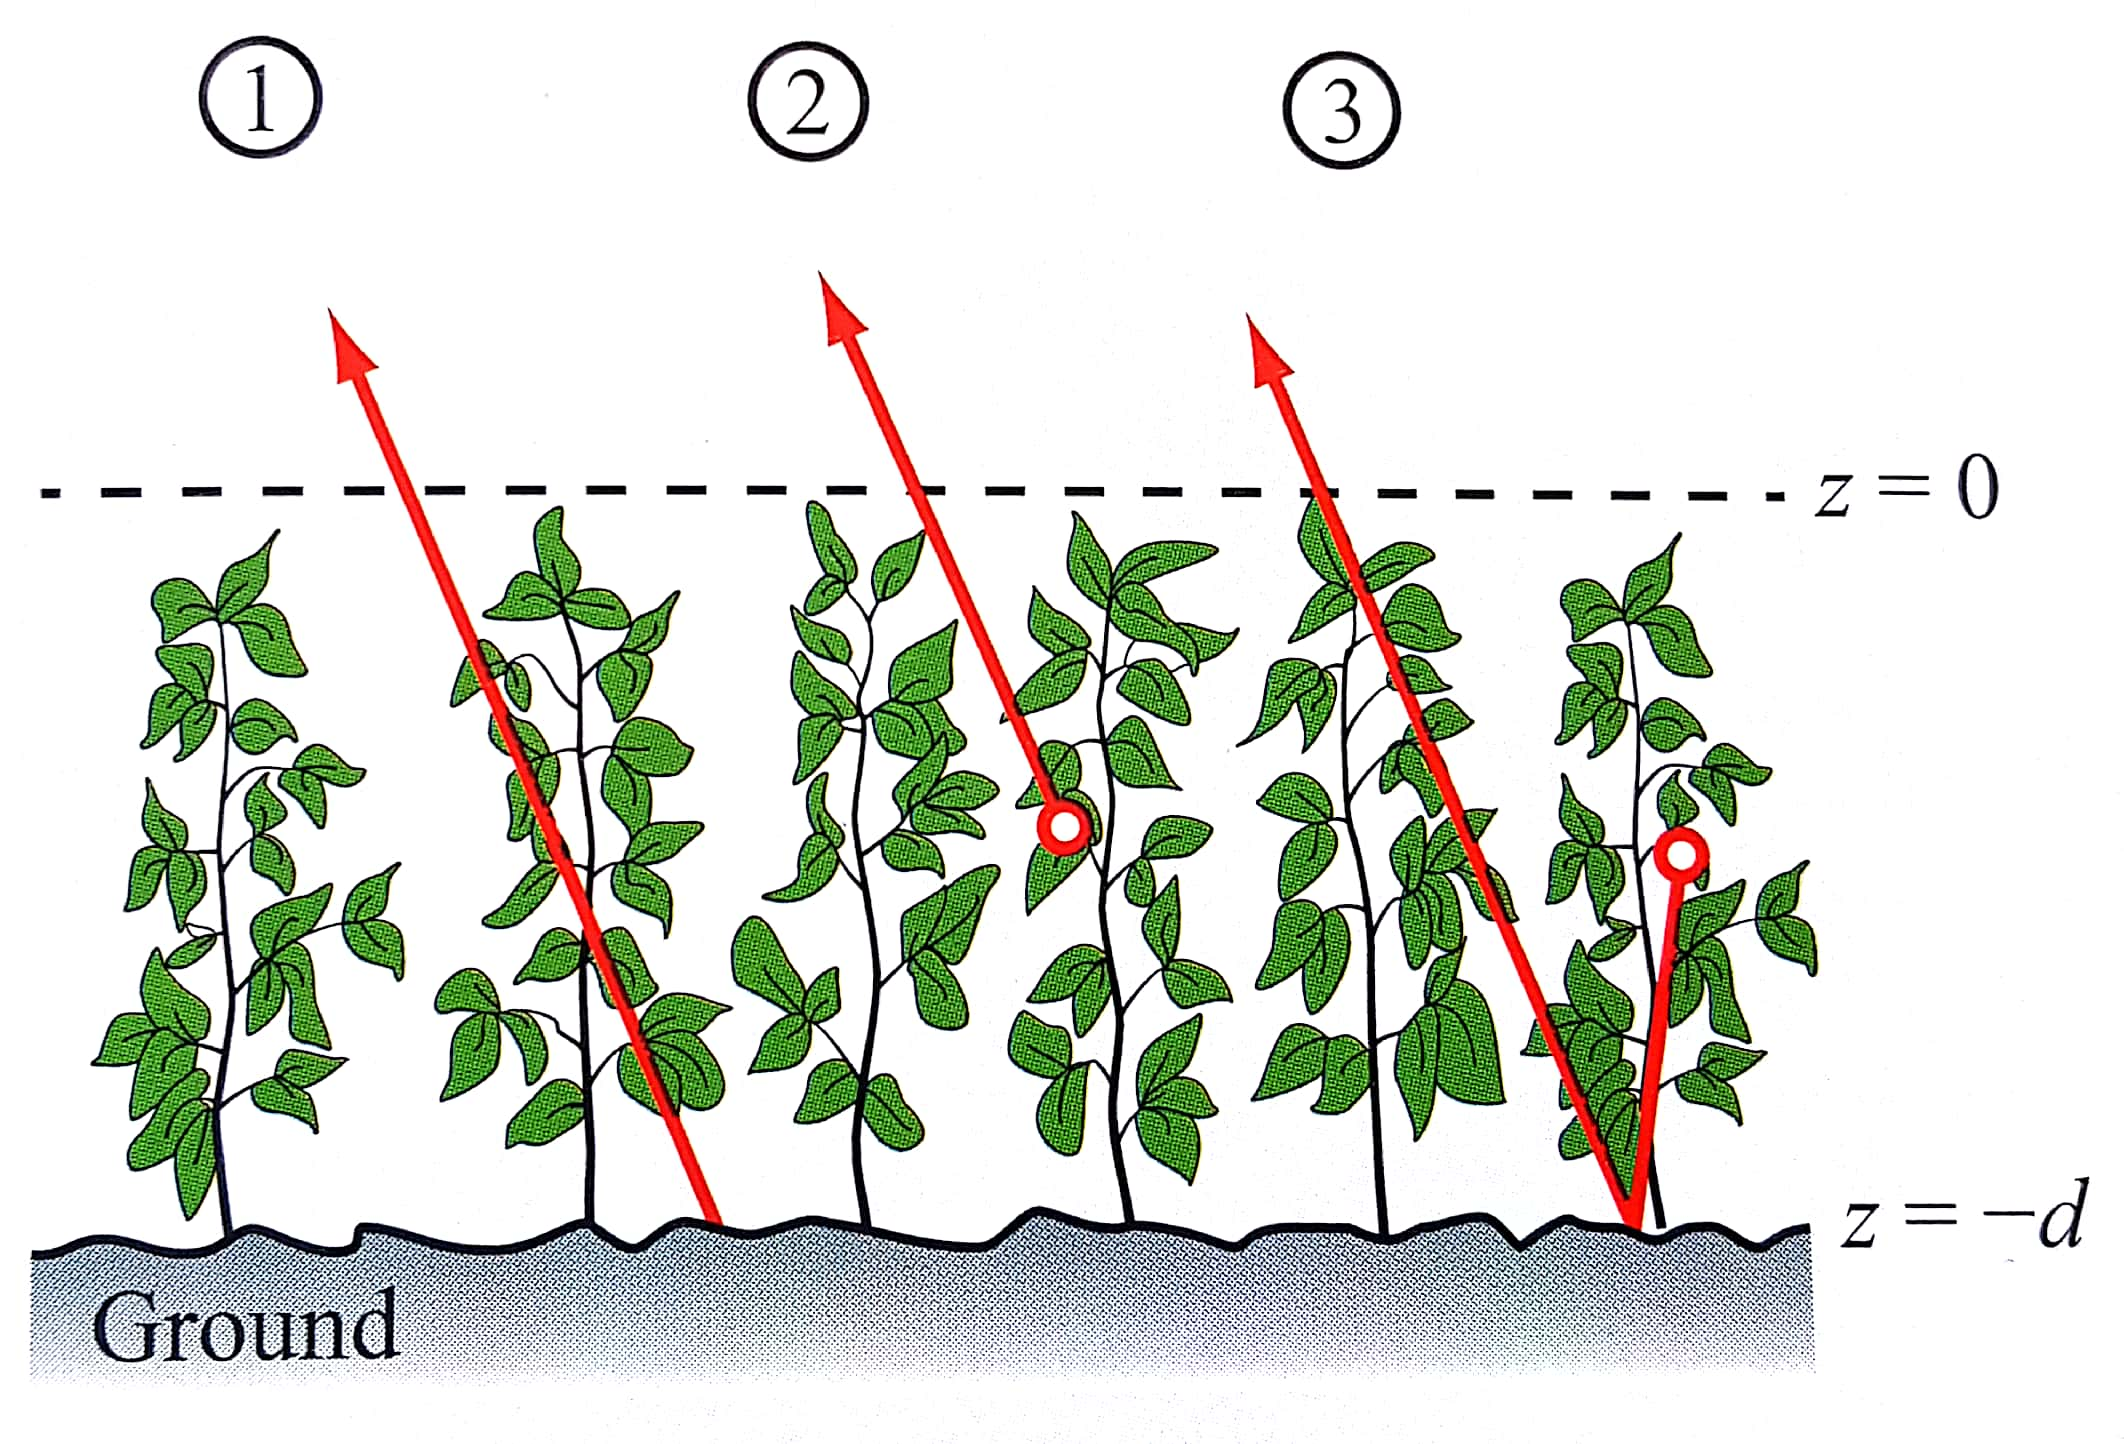
\includegraphics[width=.4\linewidth]{Figures/ZRT.jpg}
	\caption{Basic emissivity model takes into account surface emissivity, vegetation emissivity, and downward reflected vegetation emissivity. \cite{ulaby_fung_moore_1986}}
	\label{fig:zrt}
\end{figure}

The above model takes into account the ground emissivity, the vegetation emissivity, and the downward vegetation emissivity reflected off of the ground as seen in figure \ref{fig:zrt}. Higher order models take into account atmospheric emissivity and reflections, . Using the ZRT, the soil emissivity can be solved for. Soil emissivity is related to its dielectric constant as well as other surface parameters such as surface roughness. Once the dielectric constant of the soil is estimated, soil moisture content can be found using a simple dielectric model. All of these independent variables can be solved for either using other measurements at different frequencies, polarities, or incidence angles, or by utilizing tertiary datasets. Since our radiometer is only measuring a single frequency and polarization, tertiary parameters must be determined from outside data-sets. In an attempt to increase the accuracy of our radiometer system, the ZRT model will be derived as a function of the frequency and advanced parameter estimation techniques will be applied on the measure power spectral density. For example, a least squares parameter estimation technique could optimize the parameters of the ZRT model to fit the the measured power spectral density. It is expected that with this method alone, it will not be possible to eliminate every variable without resorting to tertiary data-sets. However, it is expected that this could lead to more accurate estimation of soil moisture content.
\end{enumerate}

\subsubsection{Attitude Determination}

Depending on the achieved directionality of the antenna, it may be important to determine the actual attitude of the payload during the experiment to obtain an accurate map of the ground below. If a fairly non-directional antenna is chosen, then the attitude can safely be assumed to be always NADIR pointing. Sill, an IMU might still be included as modern MEMS IMU's are small, cheap and power efficient. Determining attitude from a 9-DoF accelerometer-gyroscope-magnetometer sensor is well explored in literature. Sensor fusion based on statistical methods or Kalman filtering is so commonplace that it could almost be considered trivial. A Kalman filter based on pendulum dynamics to model the balloon payload will be implemented to fuse the 9-DoF measurements and extract the current attitude. It is expected that this method will be more than accurate enough to account for minor attitude variations given the antennas expected beam-width. \cite{Vujicic2016} \cite{Estimation2017} \cite{Rhudy2017} \cite{Chow} \cite{Wan}

\begin{figure}[h!]
	\centering
	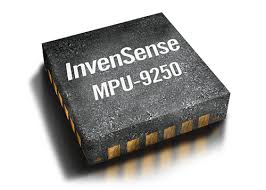
\includegraphics[width=.4\linewidth]{Figures/IMU.jpg}
	\caption{MPU9250 is a small modern low cost 9-DoF IMU}
	\label{fig:imu}
\end{figure}

\subsubsection{Thermally Controlled Noise Source}

Hybrid radiometers function by comparing the measured noise temperature to that of a known noise source. Noise sources usually take the form of a simple resistor at a specific temperature. A higher temperature will give better dynamic range to the radiometer measurements. Due to the harsh and changing thermal environment at high altitudes, our radiometer requires a thermally controlled noise source. This will take the form of a precision resistor wrapped in a NiCr heating element and insulation. A thermistor will provide feedback into a control system to keep the noise source at a constant temperature throughout the flight. The thermal mass of the resistor is quite low, so it is expected that the overall power consumption of the active thermal system will also be quite low. Power measuring circuitry will be included to monitor the payloads power consumption to ensure that the allotted 30 Wh of power will not be exceeded.

\subsubsection{Experimental Procedures}

The experimental procedure for our payload is broken down into three phases, pre-flight, flight, and post-flight operations.

\begin{enumerate}
    \item Preflight Operations: After the instrument is constructed, it is vital that a calibration is performed. At minimum, a two point calibration is required to characterize the instrument. One easy calibration point is achieved by pointing the antenna at a clear sky. This exposes the antenna only to the microwave background radiation, which is at a known temperature of 2.75 \textdegree K. The other calibration point will be achieved by constructing a thermally controlled calibration black-body. The antenna will be placed in the calibration rig, which will be thermally controlled and coated in a layer of microwave absorbing material. The physical temperature will then be varied to provide a hot calibration point. Calibration will be performed in the weeks before launch; no preparation or calibration procedures are required on launch day. Preflight operations on launch day will consist of simply plugging in the payload, fixing it on the gondola, and confirming payload operation.
    \item Flight Operations: The payload will begin taking measurements immediately after launch. This will be done because it is possible to measure or infer the physical temperature and characteristics of the ground surrounding the launch area. This can give us another potential calibration point and confirm the instruments accuracy on launch day with ground based measurements. The payload will take measurements during ascent and after apogee until either the mission is terminated or until 30 Wh of power consumption has been measured. The payload will then enter a low power sleep mode. The payload will save collected data locally for post processing at a later date. Only basic payload diagnostics and health data will be transmitted to the ground via the on-board gondola communication system. The data rate utilized by our payload is expected to be very low.
    \item Post-Flight Operations: Once the payload has been recovered and returned to the team, the data will be post processed.
\end{enumerate}

\subsection{Project Management}

\subsubsection{Technical Risk Assessment}

There are several points of risk, both human and technical, with the proposed payload. 

\begin{enumerate}
\item Human
\begin{enumerate}

\item Workload: Currently there is only two dedicated team members on CHARM, although we are also getting a significant amount of guidance from professor Jim Wight and professor Bruce Burlton. This is mainly due to the difficulty in recruiting members with sufficient knowledge of electronics and microwave systems. We are confident however that we can achieve the mission objectives laid out in this proposal.

\item Funding: It can be difficult to fund-raise enough to fully support the project. It is expected that the payload will be able to be constructed given the expected price of the components and given the funding and support received from the Carleton University and its faculty. There is some risk inherit if higher quality and low-noise components are required however.

\end{enumerate}

\item Technical and Environmental
\begin{enumerate}

\item Space Constraints: The payload requires a NADIR pointing antenna that extends out of pelican case. It is desired that the antenna is at least somewhat directional to achieve good ground resolution. There is a risk that the payload will not be able to be built within the allotted space. In this case, the payload should be redesigned to utilize a higher frequency or smaller and less directional antenna.

\item RF Interference: RF interference can greatly effect radiometers. Even low power side-bands can ruin radiometer measurements. Top of the line radiometer systems utilize several different radiometers at several frequencies to attempt to minimize the effect of RF interference. Since our payload only measures a single frequency, RF interference could prevent measurements.

\item Achieved Gain: Radiometer systems require very high gain amplifiers to measure low power noise being emitted from the earth's surface. If we cannot achieve a high enough gain or low enough noise figure, then it is possible that measurements may not be possible.

\item Calibration: Calibrating radiometer systems is non-trivial and usually involves the use of liquid nitrogen. There is a risk that the system will not be able to be properly calibrated.

\item Radiative Transfer Model: The single frequency radiometer proposed relies on tertiary data-sets to invert the transfer model and solve for soil moisture content. There is a risk that accurate estimations of soil moisture content will not be able to be determined due to the quality of the measurements, tertiary data-sets, or the models. In this case, the instrument could be quantified by generating an empirical model.

\item Thermal Environment: The thermal environment is quite harsh at high altitudes. Microwave components are quite susceptible to varying thermal conditions, and it is possible that measurements will be sufficiently degraded once high altitudes are reached. Passive thermal control is planned on everything but the noise reference.

\end{enumerate}
\end{enumerate}

\subsubsection{Team Structure}
There are currently two members on the CHARM team. Professor Bruce Burlton is acting as our faculty endorsement. We are also receiving a significant amount of help and guidance on the microwave design from professor Jim Wight.

\begin{enumerate}
\item Jacob Booth is responsible for data analysis, digital electronics design, attitude determination, the thermal reference control system, main controller software, and construction of the mechanical elements of the antenna .

\item David Bascelli is responsible for the radiometer RF section, antenna design, antenna construction, FPGA software, and digital signal processing of the power spectral density.

\end{enumerate}

\newpage

\subsubsection{Project Time-line}

A project time-line has been created and can be seen in table \ref{tab:timeline}.

\begin{table}[H]
	\centering
	\vspace{0.5cm}
	\renewcommand{\arraystretch}{1.3}
	\caption{Project time-line.}
	\label{tab:timeline}
	\begin{tabularx}{\textwidth}{lr}
		\toprule
		Milestone & Expected Deadline\\	
		\midrule
		Acquisition of components for fall semester funding & December 14th, 2018\\
		Decision on final radiometer frequency and configuration & December 31, 2018\\
		Decision on final antenna type and size & December 31, 2018\\
		Decision on final secondary electronics & December 31, 2018\\
		Microwave component purchases  & January 30, 2019\\
		Secondary electronics schematic completion & January 30, 2019\\
		Secondary electronics PCB completion & February 30, 2019\\
		Antenna construction completed  & March 15, 2019\\
		Microwave and secondary electronics integration & March 15, 2019 \\
		Micro-controller Software Completed & May 15, 2019\\
		FPGA Software Completed & May 15, 2019\\
		Calibration Rig Completed & May 15, 2019\\
		Calibration Performed & June 15, 2019\\
		Payload completed & July 15, 2019\\
		Testing and Validation & July 30, 2019\\
		Launch & August, 2019\\
		Post Flight Data Analysis & September, 2019\\
		Final Report & September, 2019
		\end{tabularx}	
\end{table}


\subsubsection{Received Funding}

Our team has currently received \$800 in funding for component purchases in the fall semester from the Carleton Undergraduate Engineering Equipment Fund (CUESEF). Another application will be submitted in the Winter and Summer semesters and similar amounts of money is expected. There are several other funding opportunities available to Carleton engineering projects in the winter semester. Test equipment such and other such items are available to be used freely from Carleton University. We also have received offers of free RF components and test equipment from both Professor Jim Wight and Nagui Mikhail.

\subsubsection{Power Budget}

A preliminary power budget has been made in table \ref{tab:powerBudget}. Values have been taken from data-sheets of selected or similar components and assuming 6 hours of continuous measurement. Electronics to monitor overall power consumption and noise reference power consumption will be implemented to ensure the payload stays within the allotted 30 Wh. The power consumption of the noise reference comes from its required active thermal control. 

\begin{table}[H]
	\centering
	\vspace{0.5cm}
	\renewcommand{\arraystretch}{1.3}
	\caption{Preliminary Power Budget}
	\label{tab:powerBudget}
	\begin{tabularx}{\textwidth}{lrrr}
		\toprule
		Component & Power Consumption & Margin & Consumption + Margin \\		
		\midrule
		Micro Processor/FPGA Board			& 4.0 Wh  & 0.50  &  6.0 Wh \\ 
		Secondary Electronics and PCB's		& 2.0 Wh  & 0.30  &  2.6 Wh \\
		Low Noise Amplifier					& 6.8 Wh  & 0.10  &  7.5 Wh \\ 
		Down conversion Mixer				& 0.5 Wh  & 0.20  &  0.6 Wh \\ 
		Noise Reference						& 8.0 Wh  & 0.50  & 12.0 Wh \\ \midrule
		Total Power Consumption				&21.3 Wh  & 0.35  & 28.7 Wh
	\end{tabularx}	
\end{table}

\subsubsection{Mass Budget}

A preliminary mass budget has been made in table \ref{tab:massBudget}. Values have been taken from data-sheets of selected or similar components or estimated based on the selected materials and estimated size. 

\begin{table}[H]
	\centering
	\vspace{0.5cm}
	\renewcommand{\arraystretch}{1.3}
	\caption{Mass Budget }
	\label{tab:massBudget}
	\begin{tabularx}{\textwidth}{lrrr}
		\toprule
		Component & Expected Mass & Margin & Mass + Margin \\		
		\midrule
		Micro Processor/FPGA Board			&0.1 kg & 0.1& 0.11 kg \\ 
		Secondary Electronics and PCB's		&0.4 kg & 0.1& 0.44 \\
		Horn Antenna						&1.5 kg & 0.3& 1.95 \\ 
		Mechanical Fittings for Horn Antenna&1.5 kg & 0.3& 1.95 \\ 				
		Low Noise Amplifier					&0.3 kg & 0.1& 0.33 \\ 
		Down conversion Mixer		 		&0.3 kg & 0.1& 0.33 \\ 
		Down-sampling VCO			 		&0.3 kg & 0.1& 0.33 \\ 
		Noise Reference						&0.1 kg & 0.3& 0.13 \\
		Cables, Connectors, Fittings		&0.5 kg & 0.5& 0.75 \\
		Insulation							&0.3 kg & 0.3& 0.39 \\ 		\midrule
		Total Mass							&5.2 kg & 0.29& 6.71 kg
	\end{tabularx}	
\end{table}

\section{Conclusion}

The CHARM project will design a high altitude balloon payload to take passive microwave measurements for the purpose of measuring soil moisture content. The payload will take the form of a NADIR pointing horn antenna extending from the pelican case. A hybrid type radiometer will down-sample and convert the incoming microwave radiation and calculate a power spectral density of the microwave emissions. The radiometer will take differential measurements compared to a known thermally controlled noise source to eliminate varying gain in the amplifier as a source of error. Data will be post processed and a variation of the radiative transfer function will be used to estimate soil moisture content. Tertiary datasets of ground roughness and ground cover will be used to invert the transfer model and isolate for soil moisture content. Advanced parameter estimation techniques will also be attempted to fit the whole power spectral density to the radiative transfer function. Preliminary mass and power budgets are presented and it is expected that the proposed payload will be within the requirements set out by the competition.

%-------------------------------------------------------------------------------
% REFERENCES
%-------------------------------------------------------------------------------
\newpage
\section{References}

\bibliography{radiometer}

\end{document}

%-------------------------------------------------------------------------------
% REFERENCES
%-------------------------------------------------------------------------------
\newpage
\section{References}

\bibliography{radiometer}

\end{document}
